% ===== Control de saturación de los primarios (0-100) =====
\def\TONE{45} % más bajo = más claro (pastel)

% Colores pastel basados en primarios
\colorlet{softred}{red!\TONE!white}
\colorlet{softgreen}{green!\TONE!white}
\colorlet{softblue}{blue!\TONE!white}

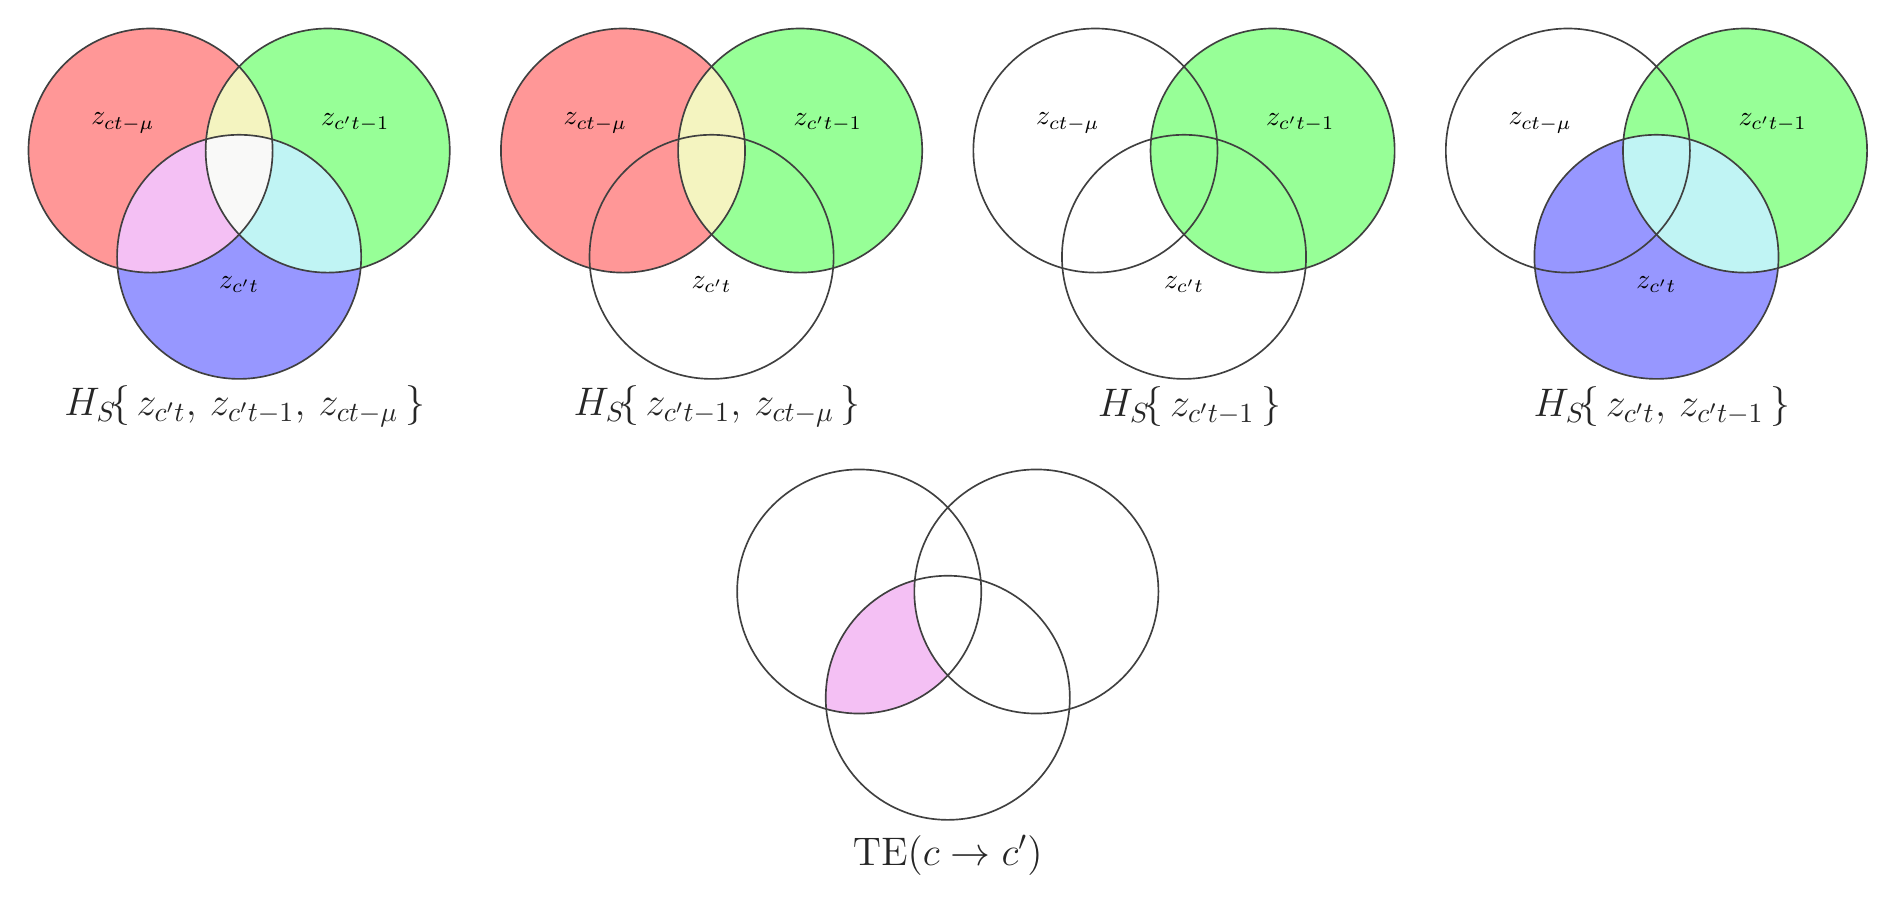
\begin{tikzpicture}[line cap=round,line join=round]
  %--- parámetros geométricos
  \def\R{1.55}
  \def\sep{2.25}
  \def\drop{1.35}

  % Etiquetas bajo los diagramas SUPERIORES
  % (aumenté 1 mm = 0.10 cm para bajarlas un poquito más)
  \pgfmathsetmacro{\UNDERPAD}{0.35}                % antes 0.25
  \pgfmathsetmacro{\yunder}{\drop + \R + \UNDERPAD}

  % Controles de la zona TE (parte inferior)
  \def\yTE{-5.6}                                   % antes -8.0 (sube ~3 mm)
  \pgfmathsetmacro{\TEeqoffsetBelow}{0.9}          % etiqueta TE debajo

  \tikzset{
    outline/.style={draw=black!75,line width=0.6pt},
    lab/.style={font=\Large, text=black!85}
  }

  % posiciones fila superior
  \def\xA{-8} \def\xB{-2} \def\xC{4} \def\xD{10}

  % === (1) ===
  \begin{scope}[shift={({\xA},{0})}]
    \coordinate (L) at (-\sep/2,0);
    \coordinate (R) at ( \sep/2,0);
    \coordinate (B) at (0,-\drop);
    \begin{scope}[blend group=screen]
      \fill[softred,   fill opacity=0.90] (L) circle (\R);
      \fill[softgreen, fill opacity=0.90] (R) circle (\R);
      \fill[softblue,  fill opacity=0.90] (B) circle (\R);
    \end{scope}
    \draw[outline] (L) circle (\R);
    \draw[outline] (R) circle (\R);
    \draw[outline] (B) circle (\R);
    
    \node[xshift=-10pt, yshift= 10pt] at (L) {$\ve{z}_{ct-\mu}$};
    \node[xshift= 10pt, yshift= 10pt] at (R) {$\ve{z}_{c't-1}$};
    \node[xshift=  0pt, yshift=-10pt] at (B) {$\ve{z}_{c't}$};
    
    \node[lab, align=center] at (0,-\yunder)
      {$\;H_S\!\bigl\{\, \ve{z}_{c't},\, \ve{z}_{c't-1},\, \ve{z}_{ct-\mu} \,\bigr\}$};
  \end{scope}

  % === (2) ===
  \begin{scope}[shift={({\xB},{0})}]
    \coordinate (L) at (-\sep/2,0);
    \coordinate (R) at ( \sep/2,0);
    \coordinate (B) at (0,-\drop);
    \begin{scope}[blend group=screen]
      \fill[softred,   fill opacity=0.90] (L) circle (\R);
      \fill[softgreen, fill opacity=0.90] (R) circle (\R);
    \end{scope}
    \draw[outline] (L) circle (\R);
    \draw[outline] (R) circle (\R);
    \draw[outline] (B) circle (\R);

    \node[xshift=-10pt, yshift= 10pt] at (L) {$\ve{z}_{ct-\mu}$};
    \node[xshift= 10pt, yshift= 10pt] at (R) {$\ve{z}_{c't-1}$};
    \node[xshift=  0pt, yshift=-10pt] at (B) {$\ve{z}_{c't}$};
    
    \node[lab, align=center] at (0,-\yunder)
      {$\;H_S\!\bigl\{\, \ve{z}_{c't-1},\, \ve{z}_{ct-\mu} \,\bigr\}$};
  \end{scope}

  % === (3) ===
  \begin{scope}[shift={({\xC},{0})}]
    \coordinate (L) at (-\sep/2,0);
    \coordinate (R) at ( \sep/2,0);
    \coordinate (B) at (0,-\drop);
    \fill[softgreen, fill opacity=0.90] (R) circle (\R);
    \draw[outline] (L) circle (\R);
    \draw[outline] (R) circle (\R);
    \draw[outline] (B) circle (\R);

    \node[xshift=-10pt, yshift= 10pt] at (L) {$\ve{z}_{ct-\mu}$};
    \node[xshift= 10pt, yshift= 10pt] at (R) {$\ve{z}_{c't-1}$};
    \node[xshift=  0pt, yshift=-10pt] at (B) {$\ve{z}_{c't}$};
    
    \node[lab, align=center] at (0,-\yunder)
      {$\;H_S\!\bigl\{\, \ve{z}_{c't-1} \,\bigr\}$};
  \end{scope}

  % === (4) ===
  \begin{scope}[shift={({\xD},{0})}]
    \coordinate (L) at (-\sep/2,0);
    \coordinate (R) at ( \sep/2,0);
    \coordinate (B) at (0,-\drop);
    \begin{scope}[blend group=screen]
      \fill[softgreen, fill opacity=0.90] (R) circle (\R);
      \fill[softblue,  fill opacity=0.90] (B) circle (\R);
    \end{scope}
    \draw[outline] (L) circle (\R);
    \draw[outline] (R) circle (\R);
    \draw[outline] (B) circle (\R);

    \node[xshift=-10pt, yshift= 10pt] at (L) {$\ve{z}_{ct-\mu}$};
    \node[xshift= 10pt, yshift= 10pt] at (R) {$\ve{z}_{c't-1}$};
    \node[xshift=  0pt, yshift=-10pt] at (B) {$\ve{z}_{c't}$};
    
    \node[lab, align=center] at (0,-\yunder)
      {$\;H_S\!\bigl\{\, \ve{z}_{c't},\, \ve{z}_{c't-1} \,\bigr\}$};
  \end{scope}

  % ---- Conjunto inferior (TE)
  \pgfmathsetmacro{\xCenter}{(\xA+\xD)/2}
  \begin{scope}[shift={({\xCenter},{\yTE})}]
    \coordinate (L) at (-\sep/2,0);
    \coordinate (R) at ( \sep/2,0);
    \coordinate (B) at (0,-\drop);
    \begin{scope}[blend group=screen]
      \begin{scope}
        \clip (B) circle (\R);
        \clip (L) circle (\R);
        \fill[softred, fill opacity=0.90, even odd rule] (-6,-7) rectangle (6,4) (R) circle (\R);
        \fill[softblue, fill opacity=0.90, even odd rule] (-6,-7) rectangle (6,4) (R) circle (\R);
      \end{scope}
    \end{scope}
    \draw[outline] (L) circle (\R);
    \draw[outline] (R) circle (\R);
    \draw[outline] (B) circle (\R);
  \end{scope}

  % Etiqueta TE DEBAJO del diagrama inferior
  \node[lab] at (\xCenter, {\yTE - \R - 0.9 - \TEeqoffsetBelow}) {$\mathrm{TE}(c \to c')$};

\end{tikzpicture}